\documentclass[answers]{exam}

%% Language and font encodings
\usepackage[english]{babel}
\usepackage[utf8x]{inputenc}
\usepackage[T1]{fontenc}
\usepackage{comment}
\usepackage{hyperref}
\usepackage{amsmath}
\usepackage{multirow}
% \usepackage{enumitem}
%% Sets page size and margins
\usepackage[a4paper,margin=2cm]{geometry}

%% Useful packages
\usepackage{amsmath}
\usepackage{amssymb}
\usepackage{graphicx}
\usepackage{paralist}
\usepackage{framed}
\usepackage{tikz}
\usepackage{float}
\usepackage{listings}

\tikzset{
  % define the bar graph element
  bar/.pic={
    \fill (-.1,0) rectangle (.1,#1) (0,#1) node[above,scale=1/2]{$#1$};
  }
}
\usetikzlibrary{matrix}
\setlength\FrameSep{4pt}
\title{\textbf{Probability \& Statistics\\ Project}} 
\author{Shamsa Hafeez Dawoodani - sd06162\\ Alisha Momin - am05757\\
Umema Zehra - uz05607}
\begin{document}
\maketitle
\begin{center}
    
\includegraphics[scale=1.5]{page1.PNG}
\end{center}
\newpage
\noindent \hrulefill
\section{Random Walk}
\begin{framed}

\textbf{Solution:\\}
\textbf{Task 1.1:\\}
This function that takes in two parameters n and p. Where n is the number of steps left or right, as dictated by the probabilities and p is the probability of steps in the right direction. In our code, the total number of experiment were led for 100 steps each is 1000. We set the starting position equal to 0. Over here we generated an array, filled with zero, of the size of experiment i.e 1000. Our function generates a number in the range of 0.0 to 1.0 randomly till $h<n$. Then it checks if $x <$ P(moving right) then it will move in a right direction otherwise it will move in left direction. We store the expected position in a $position\_list$ and then add all the element of $position\_list$ in total and then we found the average of the total and store that in numpyarray.The experiment is rehashed several time using iteration and we created one figure containing 4 histograms with a different number of bins i.e. 10, 25, 55, 80 bins for the better result.\\
\begin{center}
    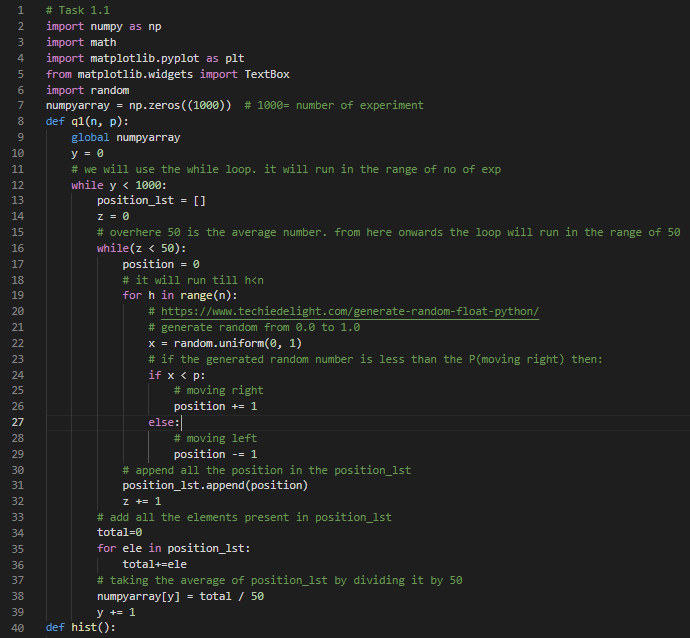
\includegraphics[scale=0.7]{task1.1a.PNG}\\
    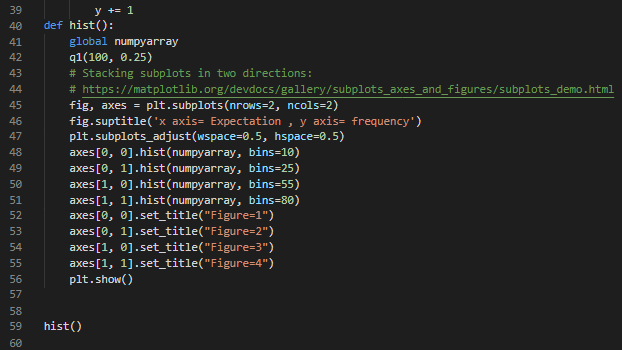
\includegraphics[scale=0.7]{task1.1b.PNG}
\end{center}
When we put n=100 and p=0.5, it give us the expected value of zero that is:  \begin{center}
    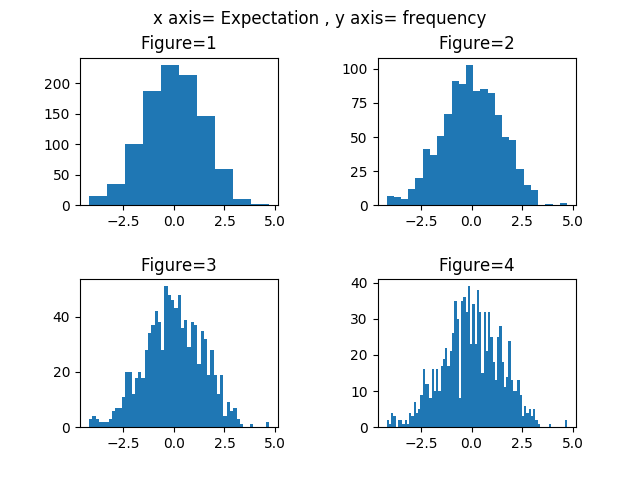
\includegraphics[scale=0.7]{hist1.1_p=0.5.png}
\end{center}
When we put n=100 and p=0.25, it give us the expected value with the most probability of moving in left direction: \begin{center}
    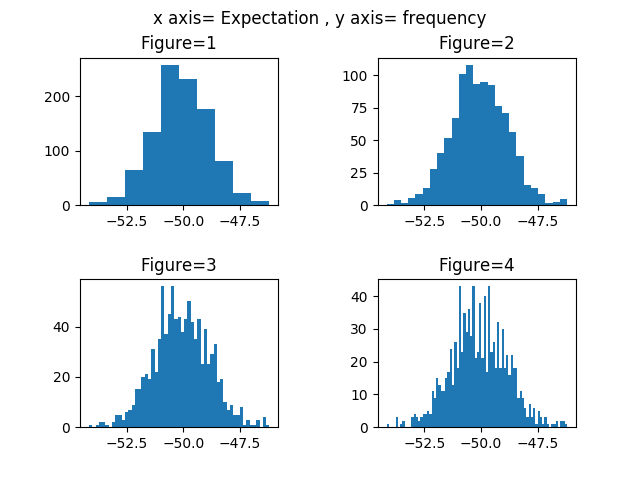
\includegraphics[scale=0.7]{hist1.1_p=0.25.png}
\end{center}
When we put n=100 and p=0.8, it give us the expected value with the most probability of moving in right direction:\begin{center}
    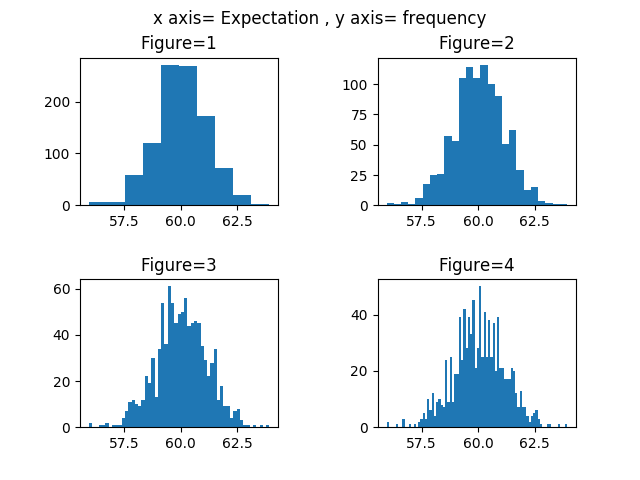
\includegraphics[scale=0.7]{hist1.1_p=0.8.png}
\end{center}
\end{framed}
\begin{framed}
\textbf{Task 1.2:\\}
This function that takes in two parameters n and p. Where n is the number of steps left or right, as dictated by the probabilities and p is the probability of steps in the right direction. In our code, the total number of experiment were led for 100 steps each is 1000. We set the starting position equal to 0. Over here we generated an array, filled with zero, of the size of experiment i.e 1000. Our function generates a number in the range of 0.0 to 1.0 randomly till $h<n$. Then it checks if $x <$ P(moving right) then it will move in a right direction otherwise if the current position is greater than zero and $x\geq p$ then it will move in left direction. We store the expected position in a $position\_list$ and then add all the element of $position\_list$ in total and then we found the average of the total and store that in numpyarray.The experiment is rehashed several time using iteration and we created one figure containing 4 histograms with a different number of bins i.e. 10, 25, 55, 80 bins for the better result.
\begin{center}
    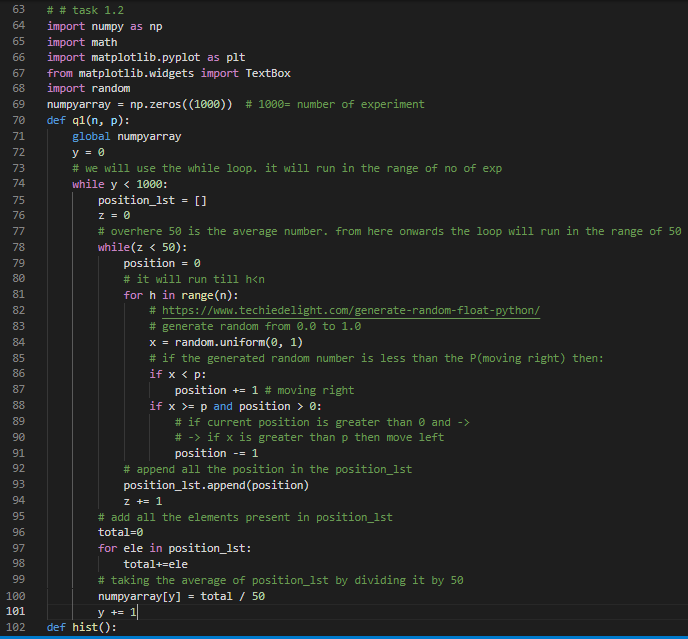
\includegraphics[scale=0.7]{task1.2a.PNG}\\
    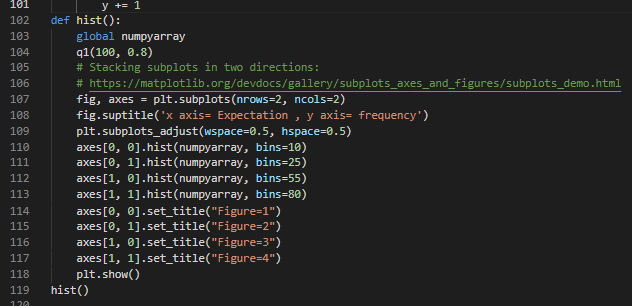
\includegraphics[scale=0.7]{task1.2b.PNG}
\end{center}
When we put n=100 and p=0.5, p=0.25 and p=0.8 respectively give us the expected value:
\begin{center}
    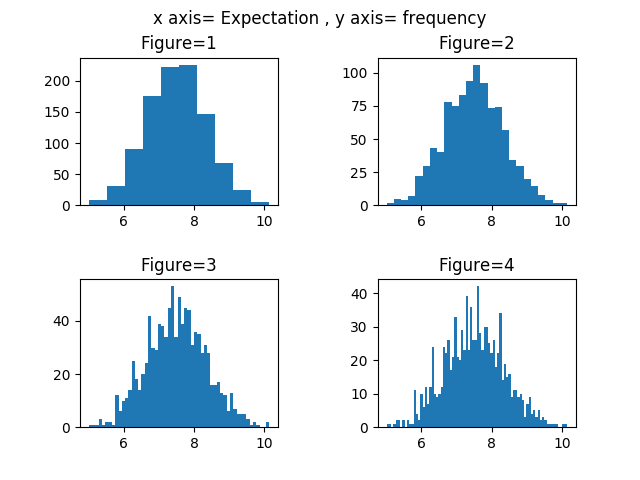
\includegraphics[scale=0.6]{hist1.2_p=0.5.png}\\
    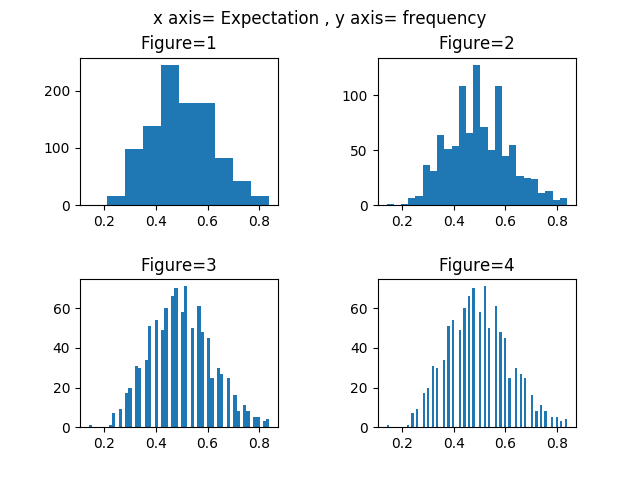
\includegraphics[scale=0.6]{hist1.2_p=0.25.png}\\
    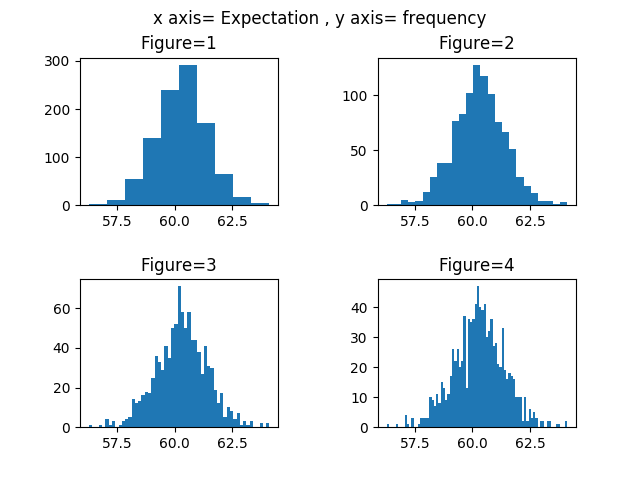
\includegraphics[scale=0.6]{hist1.2_p=0.8.png}
\end{center}
\end{framed}
\begin{framed}
\textbf{Task 1.3:\\}
This function that takes in 4 parameters, the start position of object 1,  the start position of object 2,  the probability of object 1 to move right and the probability of object 2 to move right. In our code, the total number of experiment were led for 100 steps each is 1000 with the average of 50. Over here we generated an array, filled with zero, of the size of experiment i.e 1000. Our function generates two number in the range of 0.0 to 1.0 randomly. Then it checks 4 if conditions and run until $i_{1}$is not equal to $i_{2}$. Once the position of both the objects are equal i.e $i_{1}$is equal to $i_{2}$ then the while loop is break. We store the steps in a list and then add all the element of list in total and then we found the average of the total and store that in numpyarray.The experiment is rehashed several time using iteration and we created one figure containing 4 histograms with a different number of bins i.e. 10, 25, 55, 80 bins for the better result. \\
Note: This function works similarly like task 1.1. we only modify few conditions for two objects along with their 2 probability of moving right.
\begin{center}
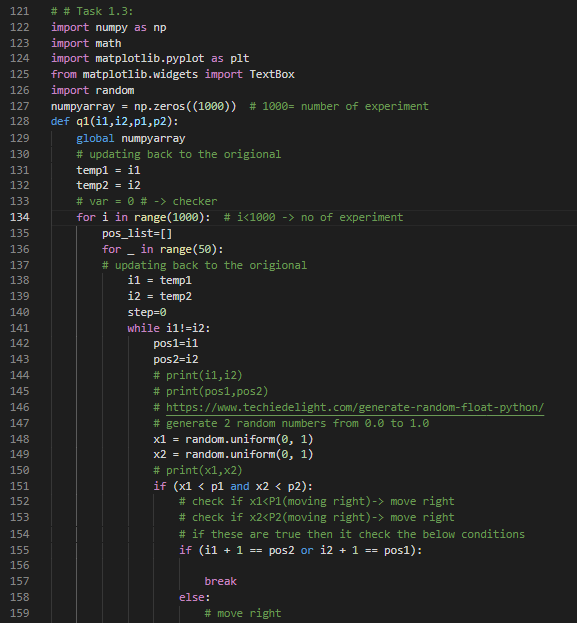
\includegraphics[scale=1]{task1.3_a.PNG}\\
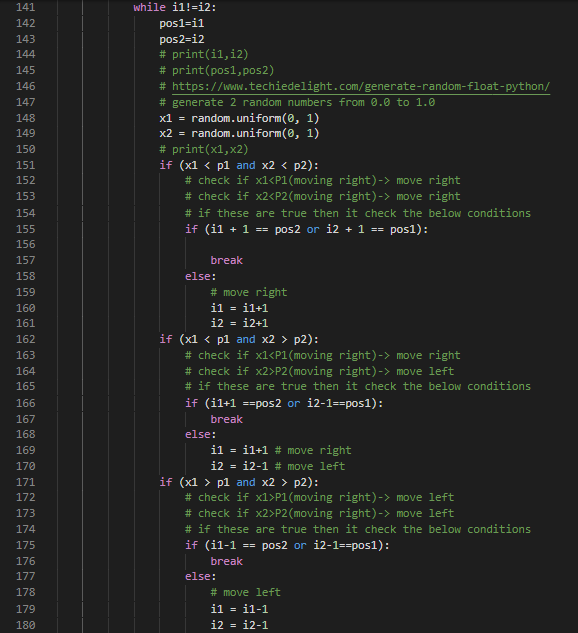
\includegraphics[scale=1]{task1.3_b.PNG}\\
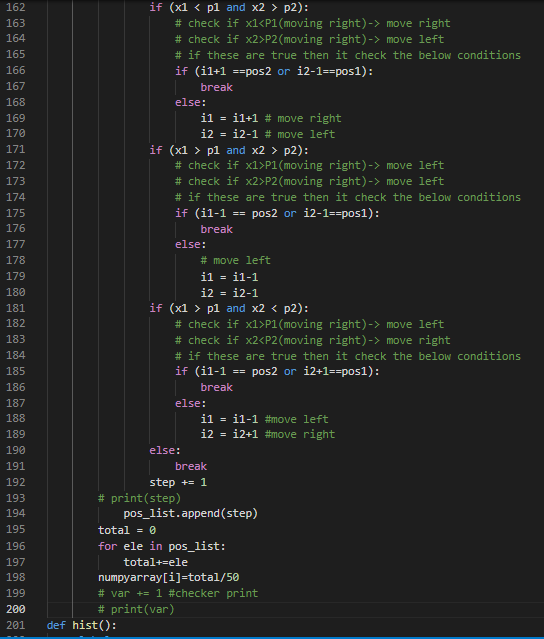
\includegraphics[scale=1]{task1.3_c.PNG}\\
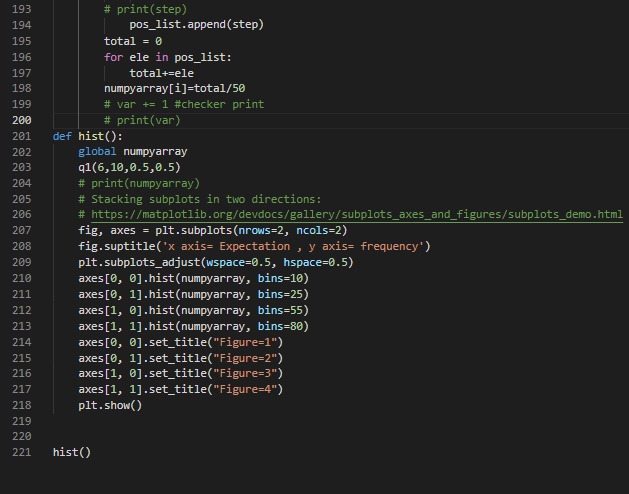
\includegraphics[scale=0.7]{task1.3_d.PNG}
\end{center}
When we put $i_{1}$=6 ,$i_{2}$=10 and $p_{1},p_{2}$=0.5
\begin{center}
    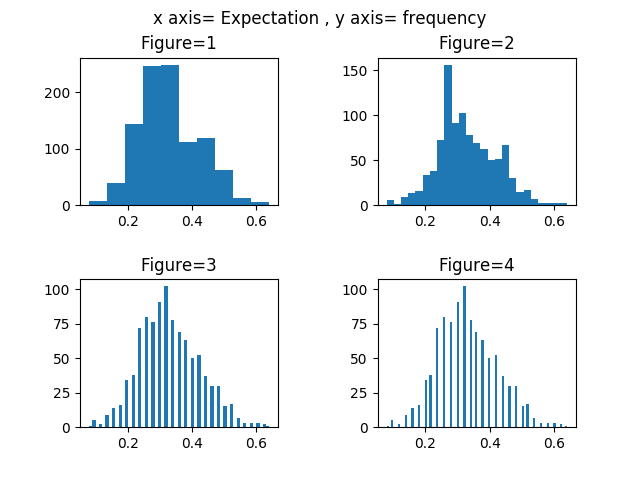
\includegraphics[scale=0.75]{hist1.3_a.png}
\end{center}
When we put $i_{1}$=-2 ,$i_{2}$=5 and $p_{1} = 0.9 ,p_{2}=0.5$
\begin{center}
    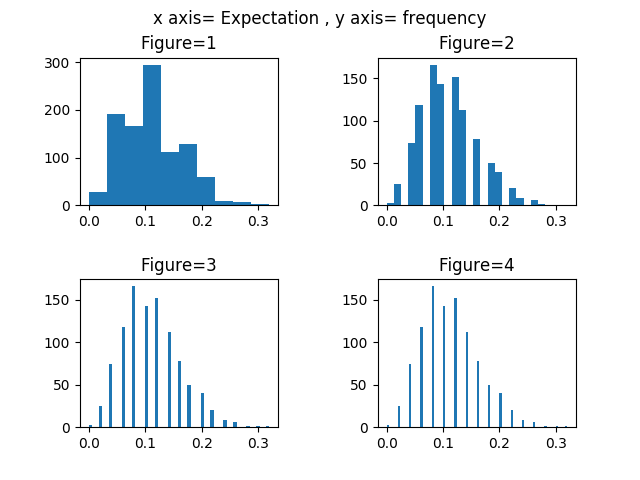
\includegraphics[scale=0.7]{hist1.3_b.png}
\end{center}
\end{framed}

\newpage
\section{Simulating Distribution}
Look at the following algebra and examine the accompanying code.\\
Let $X$ follow a uniform distribution between 0 and 1. The probability that $X$ is less than some number, $x$, is $P(X < x) = x$. Suppose we want $Y$ to follow a random distribution for which we do not have any in built functions. Let $Y$ follow the distribution $f_Y(y) = e^{-y}$ for $y \geq 0$. The following trick is used to derive the relation between X and Y. \\
\begin{figure}[H]
            \centering
            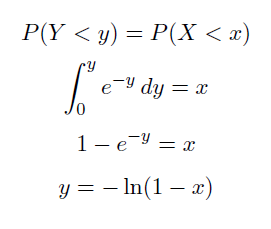
\includegraphics[width= 0.5\textwidth]{Q2_question.PNG}
        \end{figure}
        
\begin{figure}[H]
            \centering
            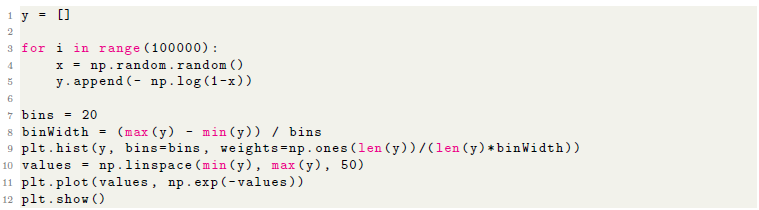
\includegraphics[width= 1.0\textwidth]{Question2_ques_code.png}
           
        \end{figure}
\subsection{} Does the code accomplish simulating the distribution? Which distribution does it follow? Try running
the code with different number of bins. Attach plots and discuss your results.\\
\begin{framed}
\textbf{Solution:\\}
Yes, the above code accomplishes the distribution.\\
\textbf{Reason:} Given that $X$ is a \textbf{Uniform Distribution} between 0 and 1 such that $P(X < x) = x$. A random number generator generates a (pseudo) Random value from the standard uniform distribution [1]. So to generate a uniform distribution between 0 and 1, we generate a random number $x$ (see Line 4). \\
Since we have found that the relation between $x$ and $y$ is : 
\begin{center}
    $y = -ln(1 - x)$ \\
\end{center}
Line 5 assure that list $y$ stores all the values of $y$. \\
Line 9 plots the histogram which represents the distribution (the blue plots in the diagram)... \\
On Line 10, $values$ consists of 50 evenly spaced values of $y$ with $min(y)$ as starting point and $max(y)$ as endpoint (2). \\
Finally, on Line 11, it plots $values$ on the $x$ axis and their corresponding values, obtained from exponential function, on y-axis such that if $y_1 \in values$, it is plotted on x axis and $e^{-y_1}$ plots on y axis. \\
So we have successfully plotted the distribution $e^{-y}$ for $y \geq 0$ as shown by the red curve. \\
Note that $y \geq 0$ is assured since the relationship between $x$ and $y$ is derived after applying the lower limit and upper limit as $0$ and $y$ respectively. 
\begin{center}
    $\int^y_0 \, \, e^{-y} \, \, dy = x$\\
    $- \Bigr[ e^{-y} \Bigr|^y_0 = x$\\
    $- (e^{-y} - e^{-0}) = x$\\
    $- e^{-y} + e^{-0} = x $\\
    $1 - e^{-y}  = x$\\
\end{center}
Now, let us also discuss the results of running the code with different number of bins. 

\begin{figure}[H] % fig 2 
    \centering
    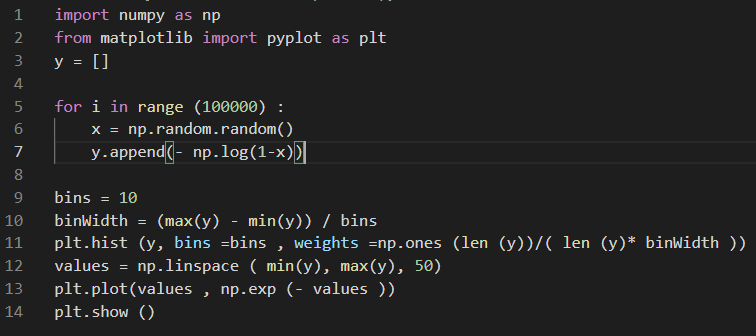
\includegraphics[width= 0.8\textwidth]{Q2.1_bins=10_code.PNG}
    \caption{Code given in Figure 1 with bins = 10}
    \vspace{2cm} 
    % fig 3
    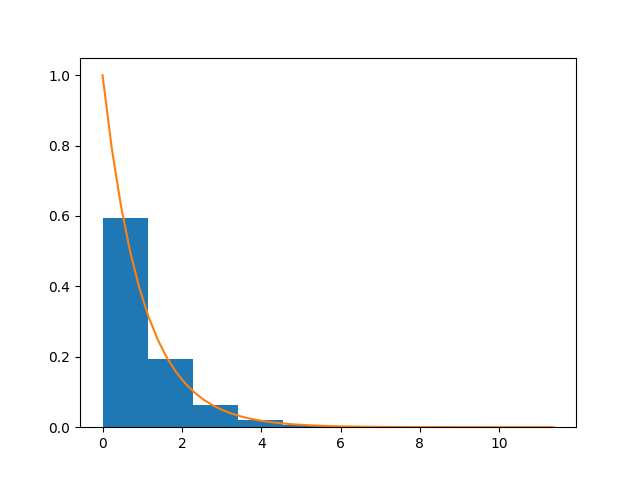
\includegraphics[width= 0.8\textwidth]{Q2.1_bins=10.png}
    \caption{Results obtained from code in figure 2 i.e., bins = 10} 
\end{figure}

\begin{figure}[H] % fig 4
    \centering
    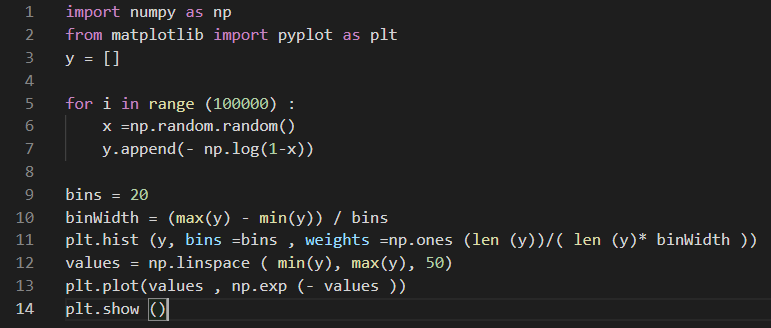
\includegraphics[width= 0.8\textwidth]{Q2.1_bins=20_code.PNG}
    \caption{Code given in Figure 1 with bins = 20}
    
     % fig 5 
    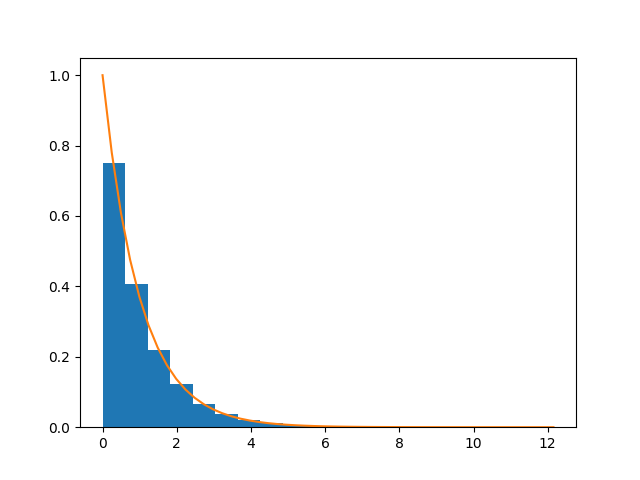
\includegraphics[width= 0.8\textwidth]{Q2.1_bins=20.png}
    \caption{Results obtained from code in figure 4 i.e., bins = 20}
 % fig 6
\vspace{1cm} 
    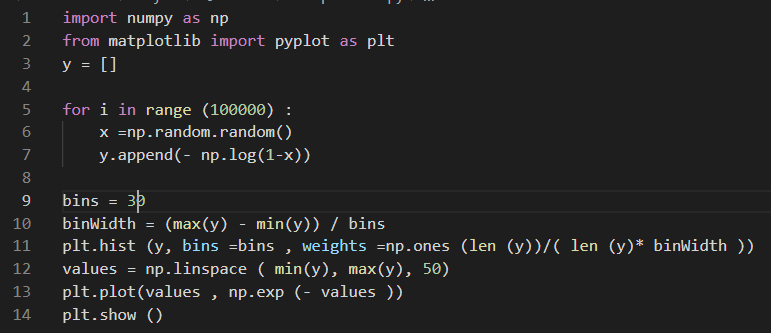
\includegraphics[width= 0.8\textwidth]{Q2.1_bins=30_code.PNG}
    \caption{Code given in Figure 1 with bins = 30}
\end{figure}

\begin{figure}[H] % fig 7
    \centering
    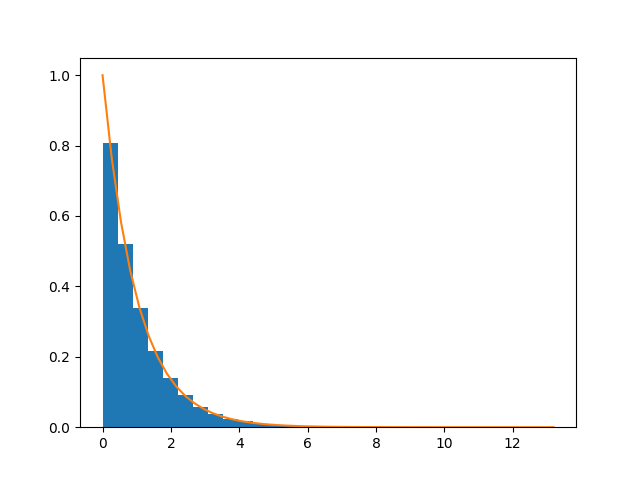
\includegraphics[width= 0.8\textwidth]{Q2.1_bins=30.png}
    \caption{Results obtained from code in figure 6 i.e., bins = 30}
    \vspace{2cm}
 % fig 8
    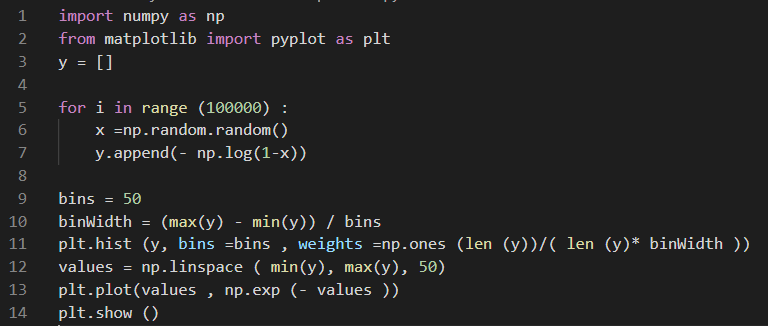
\includegraphics[width= 0.8\textwidth]{Q2.1_bins=50_code.PNG}
    \caption{Code given in Figure 1 with bins = 50}
\end{figure}

\begin{figure}[H] % fig 9 
    \centering
    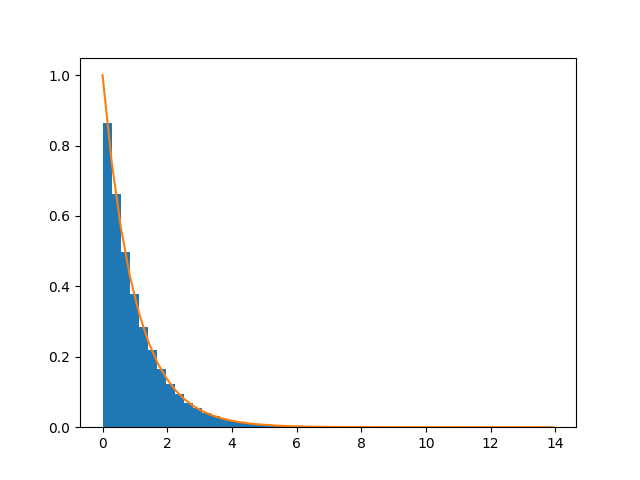
\includegraphics[width= 0.8\textwidth]{Q2.1_bins=50.png}
    \caption{Results obtained from code in figure 8 i.e., bins = 50}
    \vspace{2cm}
 % fig 10
    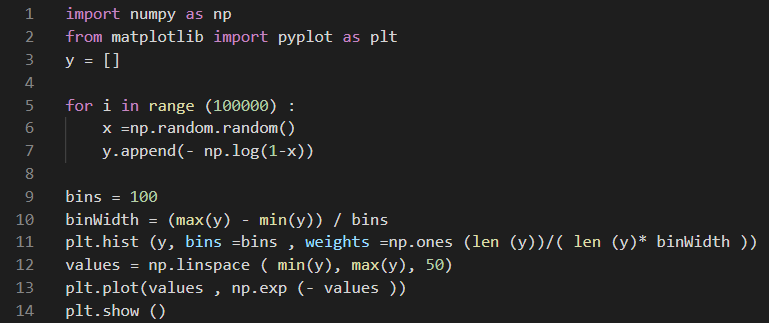
\includegraphics[width= 0.8\textwidth]{Q2.1_bins=100_code.PNG}
    \caption{Code given in Figure 1 with bins = 100}
\end{figure}

\begin{figure}[H] % fig 11 
    \centering
    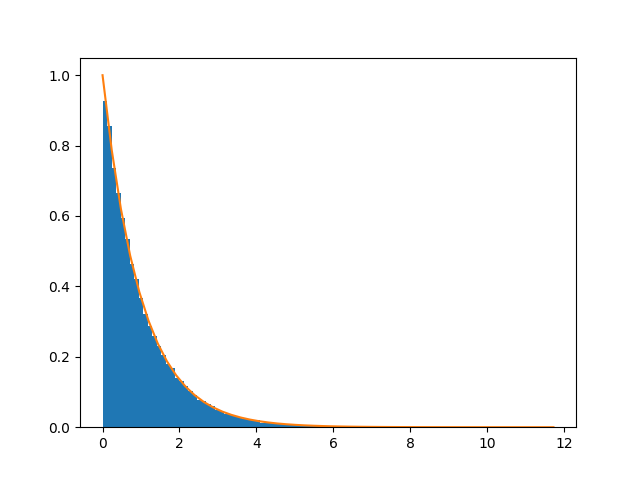
\includegraphics[width= 0.8\textwidth]{Q2.1_bins=100.png}
    \caption{Results obtained from code in figure 10 i.e., bins = 100}
 % fig 12
    \vspace{1cm}
    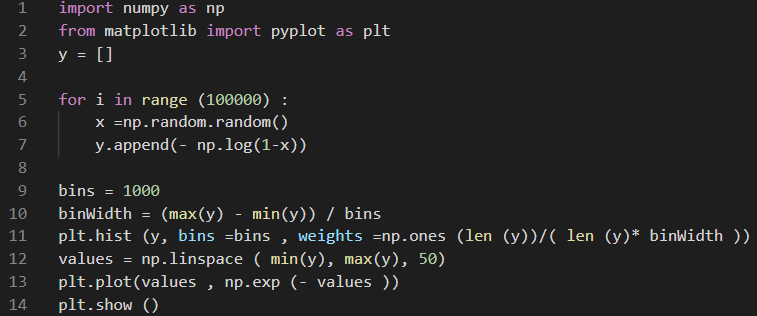
\includegraphics[width= 0.8\textwidth]{Q2.1_bins=1000_code.PNG}
    \caption{Code given in Figure 1 with bins = 1000}
\end{figure}

\begin{figure}[H] % fig 13
    \centering
    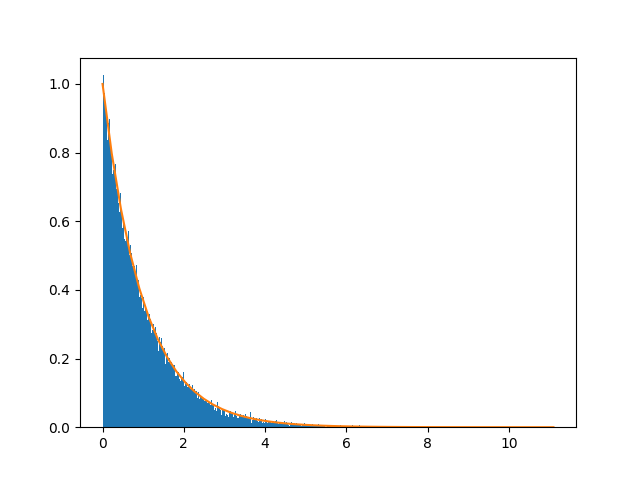
\includegraphics[width= 0.8\textwidth]{Q2.1_bins=1000.png}
    \caption{Results obtained from code in figure 12 i.e., bins = 1000}
\end{figure} 
\textbf{Finding the type of distibution:}\\
We know that a random variable $Z$ is said to have an exponential distribution with parameter $\lambda$ ($\lambda > 0$) if the PDF of $z$ is : \\

 \[
    f_Z(z) = \left\{\begin{array}{@{}lr@{}}
        \lambda e ^ {- \lambda z }& \text{for } z \geq 0\\
        0 & \text{otherwise }
        \end{array}\right\} 
  \]
By comparing the definition with $f_Y(y) = e^{-y}$ for $y \geq 0$  we can conclude that it is an \textbf{Exponential Distribution} with $\lambda = 1 $ and $Y$ is an Exponential Random Variable, \\ \\ 
\textbf{Results:}\\
First, let us try to understand what are bins. A histogram displays numerical data by grouping data into "bins" of equal width. Each bin is plotted as a bar whose height corresponds to how many data points are in that bin $^{[3]}$. \\
Now, consider the following: \\
$x \in [0, 1]$\\
$y \in [-ln(1), -ln(0)]$ Apply limit instead of 0\\
$y \in [0, \infty)$\\
So, the continuous Random variable $Y$ takes in $y \in [0, \infty)$ $^{[6]}$.\\
Since our range is now from $[0, \infty)$ it is difficult to plot 100000 possibly different values on histogram so we regularize it and divide it into bins. We divide our range into discrete number of intervals and we count how many of our samples are in each of these discrete ranges $^{[7]}$. 
This implies that, increasing the number of bins draws more bars in the histogram and makes it more precise $^{[5]}$.  

Notice that the results show that as the number of bins increases, the height of the histogram that was plotted using uniform random variable $X$ (and the relation between $x$ and $y$) , shown in blue color, traces the plot of exponential random variable, as shown in red color. This shows that we can simulate different distributions by mapping from the uniform distribution. So, yes the code accomplishes the distribution. \\

\end{framed}
%%%%%%%%%%%%%%%%%%%%%% 2.2 %%%%%%%%%%%%%%%%%%%%%%%%%%%%
\subsection{} Examine the following section of code and mathematically deduce what distribution $Y$ follows (Try working the above trick in reverse starting with the last statement). Show all required working. \begin{figure}[H]
            \centering
            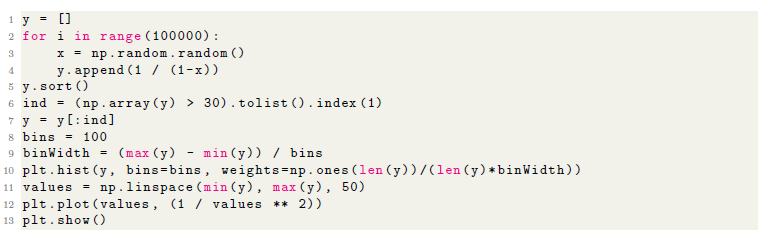
\includegraphics[width= 1.0\textwidth]{Question2.2_ques_code.png}
\end{figure}
Why are the lines 5-7 important. What does removing them do?
\begin{framed}
Let us first deduce the distribution that $Y$ follows. 
Let $X$ follow a uniform distribution between 0 and 1. The probability that $X$ is less than some number,$x$, is $P(X < x) = x$. From Figure 14 Line 4 we can find the relation between $x$ and $y$: 

$y = \frac{1}{1-x}$\\
    $1 - x = \frac{1}{y}$\\
    $x = 1 - \frac{1}{y}$\\
    $x \in [0, 1]$ and $y \in [1, y]$\\
    $x = \int^y_1 \, \, \frac{d}{dy} (1 - \frac{1}{y}) \, \, dy$\\
    $x = \int^y_1 \, \, - (\frac{d}{dy} y^{-1}) \, \, dy$\\
    $x = \int^y_1 \, \, (-1)(-1)y^{-2} \, \, dy$\\
    $x = \int^y_1 \, \, \frac{1}{y^2} \, \, dy$\\ 
    So, $Y$ follows the distribution $f_Y(y) = e^{-y}$ for $y \geq 1$ . \\
Let us now understand why Line 5-7 are important. \\
Line 5 sorts the list the list of $y$ in ascending order.  \\
For example: If $y = [ 5, 4, 80, 1 ]$ then after $y,sort()$ , $y = [1, 4, 5, 80]$ \\
Line 6 stores the index of smallest element (in the sorted list of $y$) that is greater than 30 in variable $ind$.
For example: If $y = [1, 2, 40, 80]$ so $ind = 2$\\
Line 7 updates $y$ such that sorted $y$ is sliced up till the smallest element in $y$ that is less than or equal to 30. For Example: Just before executing Line 7 $y = [1, 4, 5, 30, 80]$ and after Line 7 $y = [1, 4, 5, 30]$ \\
Its importance lies in the fact that $y = \frac{1}{1-x}$\\
So, as $x \rightarrow 1$, $y \rightarrow \infty$\\
So, if we remove Line 5 - 7 , the maximum value of $y$, can be infinitely large. \\
$max(y) \rightarrow \infty$\\
The range of $y$ has increased just because of at least a single large outcome of $y$. A zoomed out version of the graph would be obtained. As a matter of fact, the declining slope will look almost flat since the range of $y$ has increased and needs to be accommodated in the graph. In fact, the histogram seems to have been disappeared due to this reason! 
\newpage
\begin{figure}[H] % fig 16
    \centering
    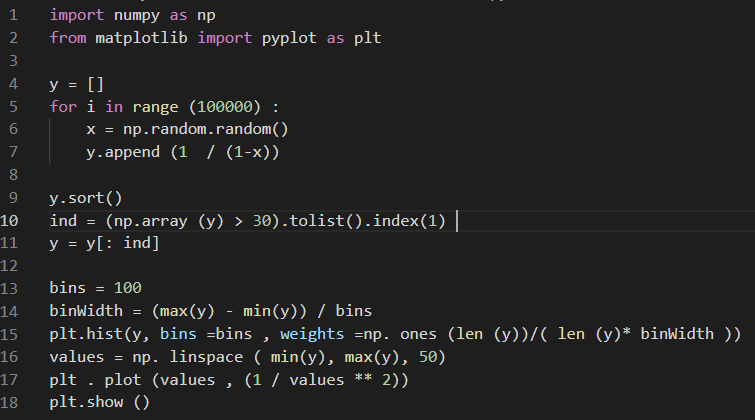
\includegraphics[width= 0.8\textwidth]{Q2.2_withLine5-7_code.PNG}
    \caption{Code with Line 5-7}
    
    \vspace{1cm} % fig 17
    
    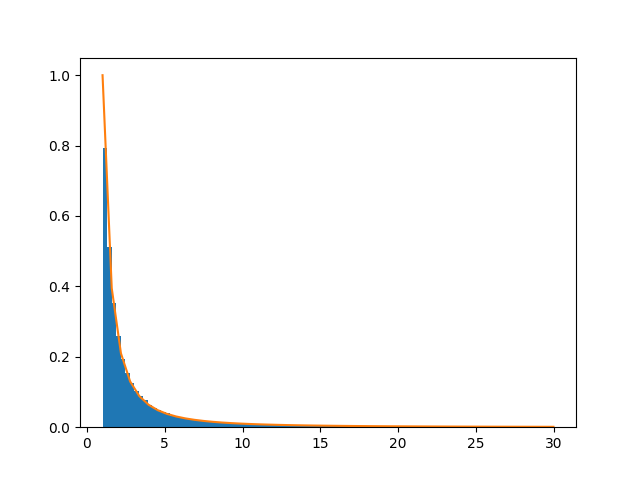
\includegraphics[width= 0.8\textwidth]{Q2.2_withLine5-7.PNG}
    \caption{Graph with Line 5 - 7 }
\end{figure}
\newpage
\begin{figure}[H] % fig 18
    \centering
    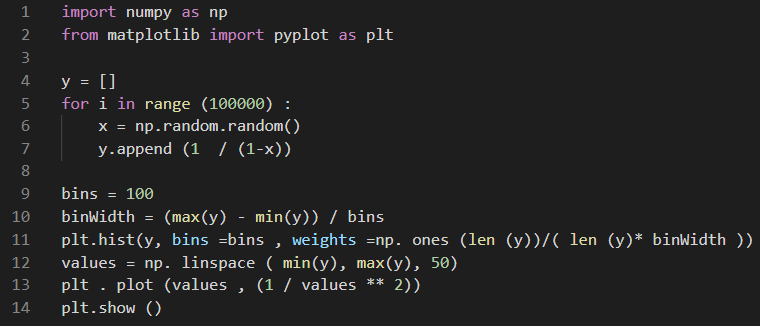
\includegraphics[width= 0.8\textwidth]{Q2.2_withoutLine5-7_code.PNG}
    \caption{Code without Line 5-7 }
    
    \vspace{1cm} % fig 19
    
    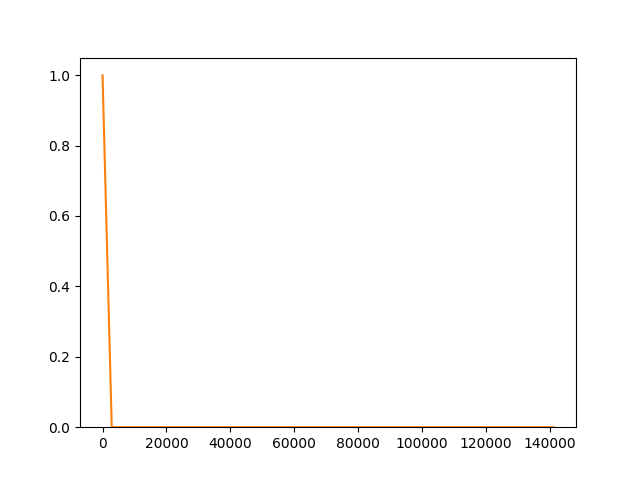
\includegraphics[width= 0.8\textwidth]{Q2.2_withoutLine5-7.PNG}
    \caption{Graph without Line 5 - 7}
\end{figure}

So, when Line 5 - 7 are removed the distribution curve does not seem to satisfy the appropriate distribution function from which it is calculated. Line 5 - 7 restricts the possible range of values of $y$ so that the histogram gives a local view of the Probability Distribution Function that justifies $f_Y(y) = e^{-y}$ for $y \geq 0$ (OR 1) 
\end{framed}

%%%%%%%%%%%%%%%%%%%%%%% 2.3 %%%%%%%%%%%%%%%%%%%%%%%%%%%%%%%%%%%%%%

\subsection{} Implement a function that returns a random variable from the distribution, \\
\begin{center}
    $f_Y(y) = \frac{1}{y^3}$ for $y \geq \sqrt{\frac{1}{2}}$ 
\end{center}
Use it to produce a histogram and line plot like the above code.\\
Implement a different function that calculates the expected value using the experiments and iterations
approach and plots the set of expected values obtained. You may need to utilize the trick pointed to
in the above lines and choose an appropriate cutoff for both of these.\\
\begin{framed}
First let us implement a function that returns a random variable from the distribution,\\
    $f_Y(y) = \frac{1}{y^3}$ for $y \geq \sqrt{\frac{1}{2}}$ \\
Let $X$ be a Random Variable that follows a uniform distribution between 0 and 1. The probability that $X$ is less than some
number, $x$, is $P(X < x) = x$. \\
Using the same trick as in $2.1$ to find the relation between $X$ and $Y$ \\
$P(Y < y) = P(X < x)$\\
$\int^y_{\sqrt{0.5}} \, \, \frac{1}{y^3} \, \, dy = x$\\
$\int^y_{\sqrt{0.5}} \, \, y^{-3} \, \, dy = x$\\
$\Bigr[ \frac{y^{-3+1}}{-3+1} \Bigr|^y_{\sqrt{0.5}} = x$\\
$-\frac{1}{2} \Bigr[ y^{-2} \Bigr|^y_{\sqrt{0.5}} = x$\\
$-\frac{1}{2} ((y^{-2}) - (\sqrt{\frac{1}{2}})^{-2}) = x$\\
$-\frac{1}{2} (\frac{1}{y^2} - 2) = x$\\
$\frac{-1}{2y^2} + \frac{2}{2} = x$\\
$1 - \frac{1}{2y^2} = x$\\
$\frac{1}{2y^2} = 1 - x$\\
$2y^2 = \frac{1}{1-x}$\\
$y^2 = \frac{1}{2(1-x)}$\\
$y = \sqrt{\frac{1}{2(1-x)}}$\\\\

Following is the code used to produce histogram and line plot like the previous parts:\\

\begin{figure}[H] % fig 
    \centering
    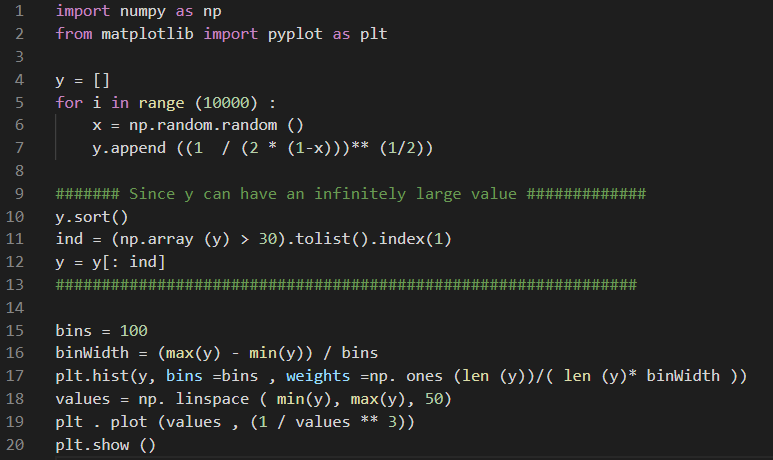
\includegraphics[width= 0.8\textwidth]{Q2.3_code.PNG}
    \caption{Code used to produce histogram and line plot for question 2.3}
\end{figure}

Notice that Line 10 - 12 are important for the same reason as Line 5 - 7 were in question 2.2. 
Since $y \geq \sqrt{\frac{1}{2}}$ in $f_Y(y)$, therefore, the list $y$ in the code above can have some values that are too large. The presence of even one such value makes it difficult to visualize the histogram as per the function provided. So, we have eliminated such large values. We are restricting the maximum possible value of $y$ such that $y \leq 30$. This is the reason why the x-axis in the histogram above graphs values from 0 to 30\\

\begin{figure}[H] % fig 
    \centering
    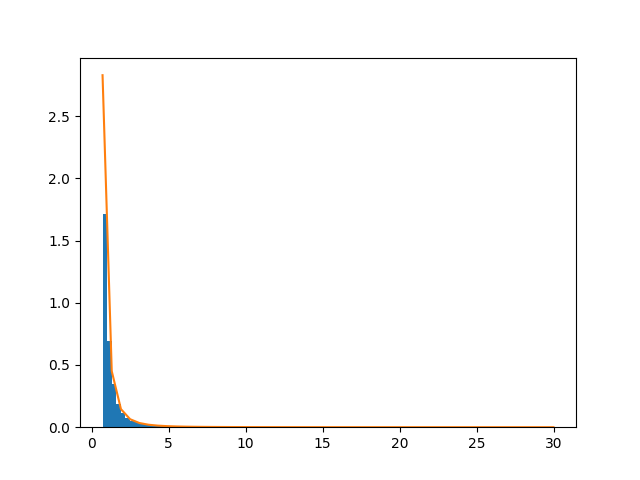
\includegraphics[width= 0.8\textwidth]{Q2.3_histogram.png}
    \caption{Histogram obtained from the distribution $f_Y(y) = \frac{1}{y^3}$ for $y \geq \sqrt{0.5}$}
\end{figure}

Finding Expected Value: \\
We know that expected value is basically the average value of a random variable. 

\begin{figure}[H] % fig 
    \centering
    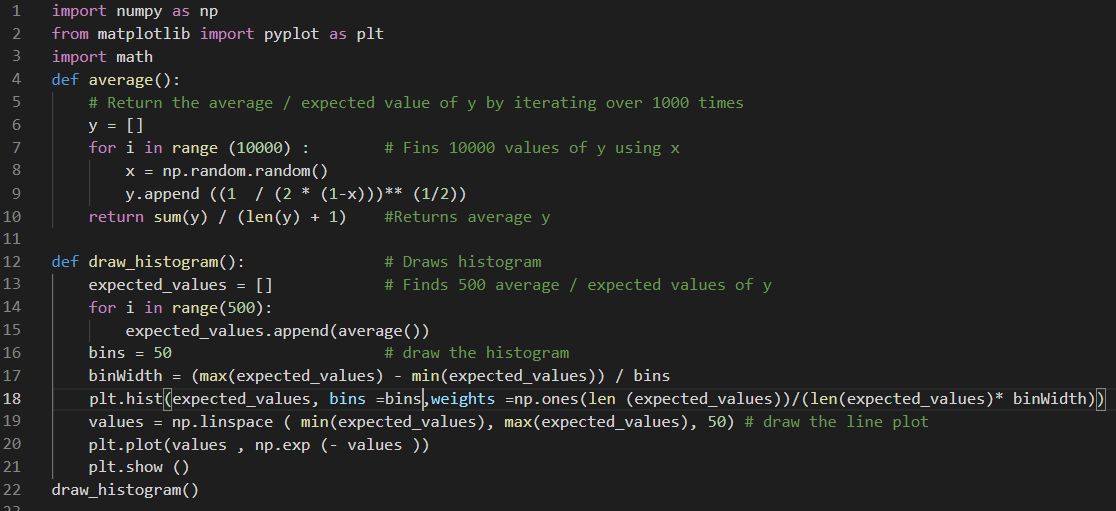
\includegraphics[width= 1\textwidth]{Q2.3_expected_value_code.PNG}
    \caption{Code used to find the expected value of $f_Y(y) = \frac{1}{y^3}$ for $y \geq \sqrt{0.5}$}
\end{figure}

This produced the following histogram: 
\begin{figure}[H] % fig 
    \centering
    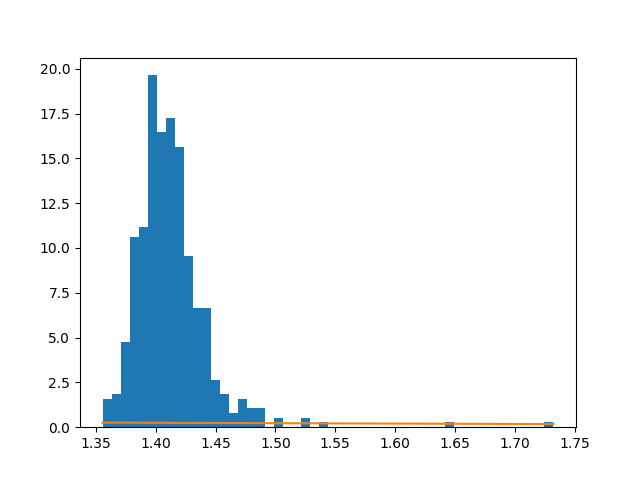
\includegraphics[width= 1\textwidth]{Q2.3_expected_value_histogram.png}
    \caption{Histogram of expected value of $f_Y(y) = \frac{1}{y^3}$ for $y \geq \sqrt{0.5}$ using experiments and iterations}
\end{figure}

Let us verify if we have obtained the correct results: \\
$E[Y] = \int^{\infty}_{\sqrt{0.5}} \, y \, \frac{1}{y^3} \, dy $\\
$E[Y] = \int^{\infty}_{\sqrt{0.5}} \, \frac{1}{y^2} \, dy $\\
$E[Y] = \Bigr[ \frac{Y^{-1}}{ -1 } \Bigr|^{\infty}_{\sqrt{0.5}} $\\
$E[Y] = \lim_{y \to \infty} \frac{-1}{y} - (- \frac{1}{\sqrt{0.5}})$\\
$E[Y] = 0 + \sqrt{2}$
$E[Y] = \sqrt{2}$\\\\
Notice that the center of the histogram that has the highest frequency is approximately 1.4. This shows that our histogram is displaying correct results 

\end{framed}

\newpage

%%%%%%%%%%%%%%%%%% 3 %%%%%%%%%%%%%%%%%%%%%%%%%%
\section{Picking a random point correctly}
%%%%%%%%%%%%%%%%% 3.1 %%%%%%%%%%%%%%%%%%%%%%%%%
\subsection{} For this question, you have to pick random points in a circle in a uniform manner. The most intuitive approach for this is usually to pick a random number, r, from the uniform distribution between 0 and R, where R is the radius of the circle. Similarly, one can pick the angle $\theta$ in a similar manner and generate x, y coordinates from them. \\
Implement a function that takes in a radius, R, and samples a large number of points in the described manner. The function should generate a scatter plot containing all the sampled points, as well as plotting a circle of the appropriate radius, Find and mention the variation in the x-coordinates as well. \\ 
\begin{framed}
    \textbf{Solution:}
    Following is our code. Note that since the question has not mentioned to keep the center of the circle into consideration we have assumed the center of the circle to be at origin. i.e., (0, 0) 
    
    \begin{figure}[H] % fig 
    \centering
    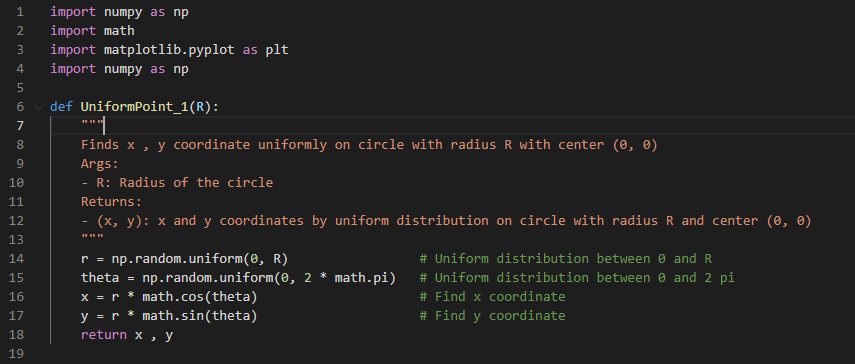
\includegraphics[width= 0.8\textwidth]{Q3.1_code_1.PNG}
     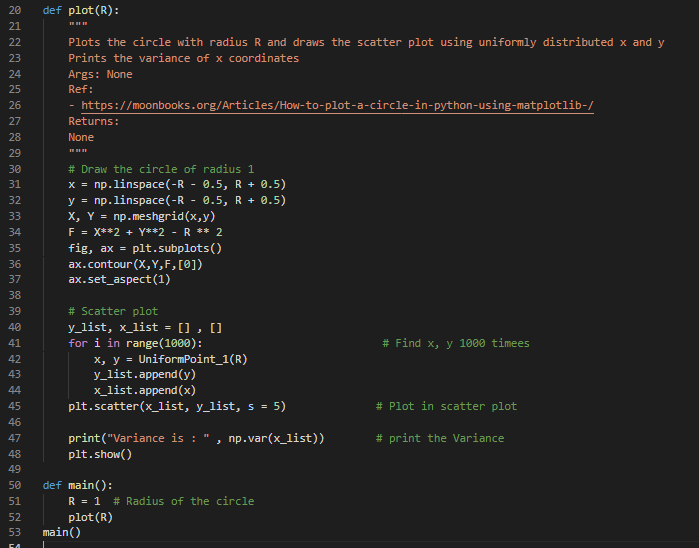
\includegraphics[width= 0.9\textwidth]{Q3.1_code_2.PNG}
     \caption{Code for 3.1}
    \end{figure}
    
    \begin{figure}[H] % fig 
    \centering
    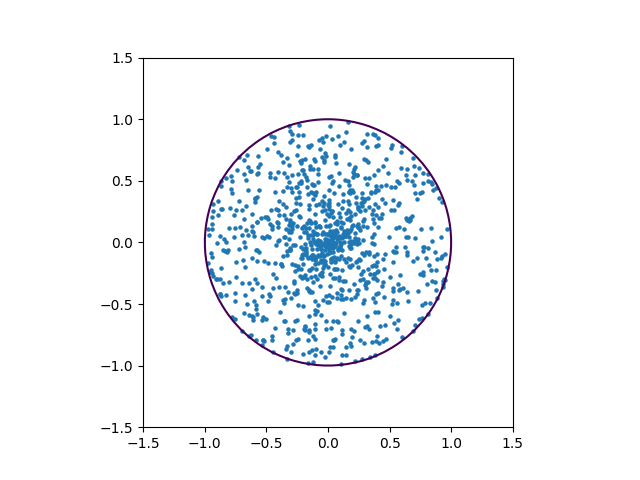
\includegraphics[width= 0.7\textwidth]{Q3.1_histogram.png}
    \caption{Scattered plot obtained using strategy mentioned in 3.1 on a circle with radius 1 centered at origin}
    \end{figure}
    
    \begin{figure}[H] % fig 
    \centering
    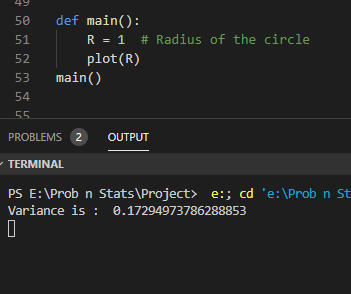
\includegraphics[width= 0.3\textwidth]{Q3.1_variance.PNG}
    \caption{variance of x-coordinates obtained using strategy mentioned in 3.1 on a circle with radius 1 centered at origin}
    \end{figure}
    
    So, the variation in the x-coordinates is 0.17294973786288853 \\
\end{framed}
\newpage
%%%%%%%%%%%%%%%%% 3.2 %%%%%%%%%%%%%%%%%%%%%%%%%
\subsection{} This, however, does not result in a uniform pick. You may spot this from the plot which should have points concentrated more towards the center rather then points being uniformly spread out across the circle. Change the number points you are plotting if you do not observe this trend. Now instead of generating $r$ and $\theta$ values we will generate x and y values uniformly. To generate random points on a
circle of radius, R, pick both x and y independently and uniformly from the range [-R, R] to obtain a point. If the distance of this point from the origin is more than R, discard it and generate a new point in its place. \\
Implement a function that takes in a radius, R, and samples a large number of points in the
described manner. The function should generate a scatter plot containing all the sampled points, as well as plotting a circle of the appropriate radius, Find and mention the variation in the x-coordinates as well. Comment on why this found variation is different or same as in the previous part.
\begin{framed}
 \begin{figure}[H] % fig 
    \centering
    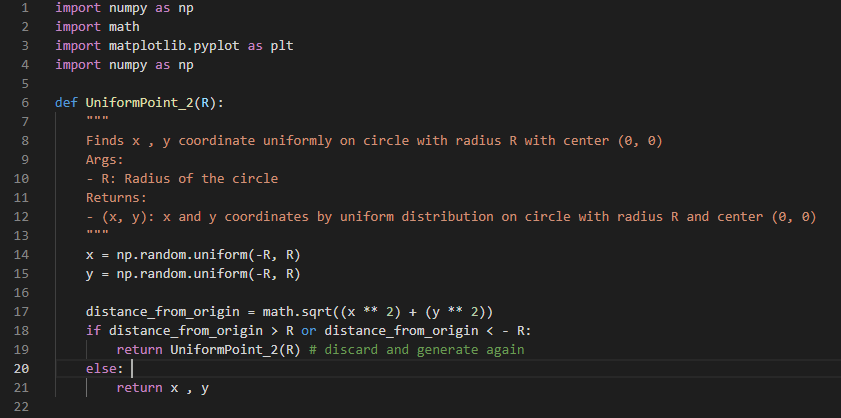
\includegraphics[width= 0.8\textwidth]{Q3.2_code_1.PNG}
     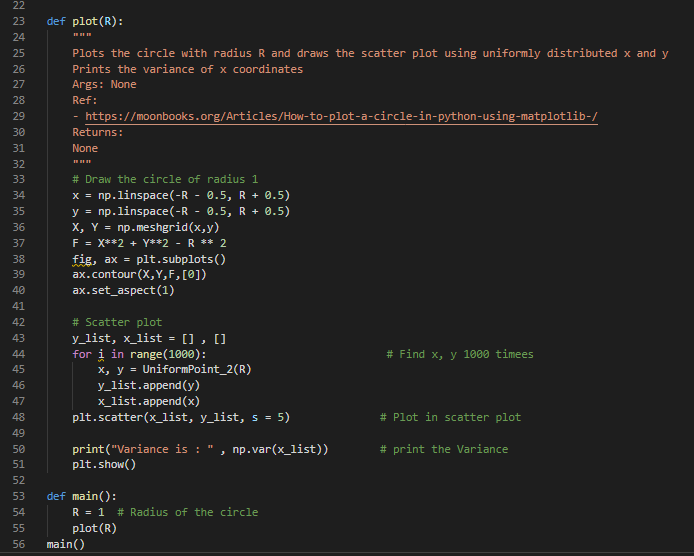
\includegraphics[width= 0.9\textwidth]{Q3.2_code_2.PNG}
     \caption{Code for 3.2}
    \end{figure}
    
    \begin{figure}[H] % fig 
    \centering
    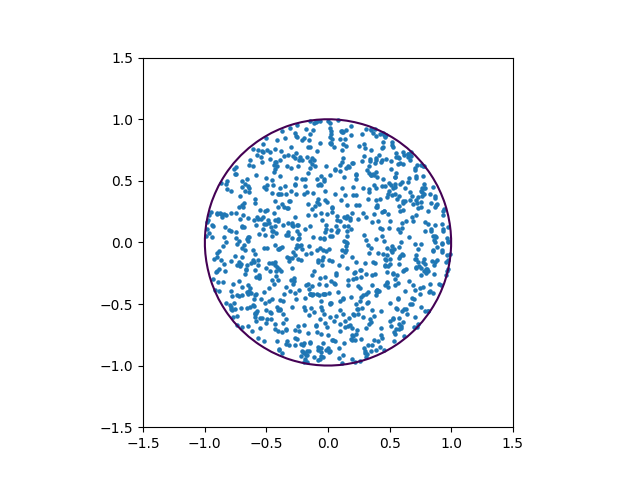
\includegraphics[width= 0.7\textwidth]{Q3.2_histogram.png}
    \caption{Scattered Plot obtained using strategy mentioned in 3.2 on a circle with radius 1 centered at origin}
    \end{figure}
    
    \begin{figure}[H] % fig 
    \centering
    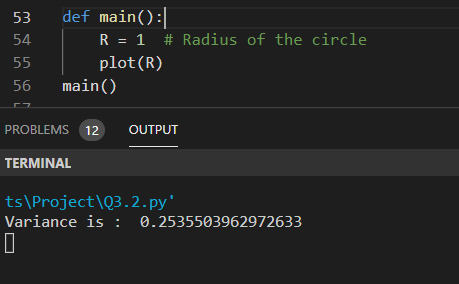
\includegraphics[width= 0.3\textwidth]{Q3.2_variance.PNG}
    \caption{variance of x-coordinates obtained using strategy mentioned in 3.2 on a circle with radius 1 centered at origin}
    \end{figure}
    
    So, the variation in the x-coordinates is 0.2535503962972633 \\

\textbf{Comment:} \\
Notice that the x coordinates' variation obtained is approximately 0.25 which is approximately 0.42 more than the variance obtained in previous approach i.e., approach used in part 3.1 (whose x coordinates' variance approximately was 0.17) although both are obtained on a circle with radius 1 centered at origin. Question arises why is that so? \\
In the first approach, points obtained are not equally spaced with respect to the center The points are the center of the circle are more dense. as we go away from the center, the density of points goes on decreasing. So this implies that the randomly generated point is more likely to be near the center than as compared to near the circumference. The points closer to the center has more probability of generation and as we go further and further away from the center this probability goes on decreasing. Thus the points obtained in 3.1 were not Uniformly distributed. However, when we picked points by a uniform random distribution of in terms of x and y coordinates the resulting points were Uniform as each point is equally likely to be obtained. Note that we are discarding a point (x, y) if it is outside the circle implying that the points to be obtained are to be limited to the area under consideration i.e., circle. The variance has increased. i.e., the degree of the spread of the data has increased increased since this is a more uniformly distributed plot \\
\end{framed}

%%%%%%%%%%%%%%%%% 3.3 %%%%%%%%%%%%%%%%%%%%%%%%%
\subsection{} To get an intuition of why the first approach does not result in a uniform pick imagine a circle of radius 1 embedded in a circle of radius 2 as shown in Fig.2. If points are picked randomly, the probability of the point lying inside the larger circle should be 4 times than the smaller one. Does this hold when the above described method to pick r and $\theta$ is used? Explain in report with working.\\
In this part, modify one or both of the ways to pick r and $\theta$ such that the points are sampled in a
uniform manner and a plot similar to that in part 2 is obtained. Implement a similar function as the
above part. The plot generated this time should contain points that are uniformly spread across the
circle. Describe how are you picking the random variables and find the variance of the x-coordinates
once again and comment on your results. \\ 
If you feeling up to it or for a bonus then you may derive the distribution from the following two facts. The probability of a point to lie inside a circle of radius, $r \leq R$ is proportional to its area. i.e. $P(r \leq R) = k \, \pi r^2$. The probability of it lying inside the outermost circle of radius, $R$ should be 1 i.e. $P(R \leq R) = 1$. \\
After finding the distribution that r follows, you may then generate the values of r appropriately by mapping from the uniform random distribution as in the previous questions. Show all mathematical working. \\

\begin{figure} % fig 
    \centering
    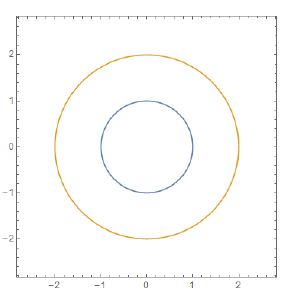
\includegraphics[width= 0.3\textwidth]{Q3.3_question.PNG}
    \caption{Comparison of area. Circles of radius 1 and 2}
\end{figure}

\begin{framed}
    \textbf{Solution:}\\
    Yes, if the above described method of $r$ and $\theta$ are used then the probability of a randomly picked point to lie in the outside circle is 4 times more than the probability of the point to lie in the smaller circle (blue one). To understand this we know that the radius of outside circle is 2. Let this radius be $r$. Consequently, the radius of the inside circle is $\frac{r}{2}$. Let A be the event of a randomly picked point (picked using randomly generated $r$ and $\theta$ as described in first approach) to lie inside/on the blue circle. Let B be the event of a randomly picked point (picked using randomly generated $r$ and $\theta$ as described in first approach) lie in the orange region.\\ \\
    $P(A) = \frac{\pi \, (\frac{r}{2})^2}{\pi \, r^2}$\\
    $P(A) = \frac{\pi \, \frac{r^2}{4}}{ \pi \, r^2}$\\
    $P(A) = \frac{1}{4} = 0.25$\\\\
    Note that since the outer circle includes the orange as well as blue region , $P(A)$ tells us that the probability of the point lying inside the larger circle is 4 times than the smaller one.\\\\

    \begin{figure}[H] % fig 
        \centering
        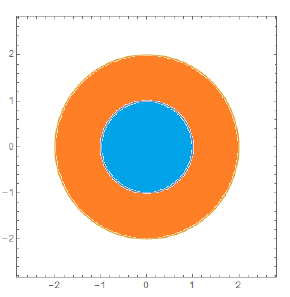
\includegraphics[width= 0.3\textwidth]{Q3.3_question_modified.png}
        \caption{Comparison of area. Circles of radius 1 and 2}
    \end{figure}

    Thus it is proved that randomly generated $r$ and $\theta$ does not result in a uniform probability \\ 
    
    %%%%%%%%%%%%%%%%%%%%%%%%%%%%%%%%%%%%%%%%%%%%%%%%%%%%%%%%%%%%%%%%%
    Given that $P(r \leq R) = k \, \pi r^2 $\\
    We want it to be uniformly distributed.So we will map it to uniformly selected $x$ such that $x \in [0, 1]$ \\
    $P(r \leq R) = k \, \pi r^2 = x$\\
    $k \, \pi r^2 = x$\\
    $r^2 = \frac{x}{k \pi}$\\
    $r = \sqrt{\frac{x}{k\pi}}$.................(i)\\
    When $r = R$ it is given that $P(R \leq R) = 1$\\
    $k\pi(R^2) = 1$\\
    $k\pi = \frac{1}{R^2}$\\
    Put in equation (i): \\ 
    $r = \sqrt{\frac{x}{\frac{1}{R^2}}}$\\
    $r = \sqrt{R^2 x}$\\
    $r = R \sqrt{x}$ \\
    
    \begin{figure}[H]
        \centering
        \includegraphics[width=1\textwidth]{Q3.3_code_1.PNG}
    \end{figure}
    
    \begin{figure}[H]
        \centering
        \includegraphics[width=1\textwidth]{Q3.3_code_2.PNG}
        \caption{Code for 3.3}
    \end{figure}
    
    \begin{figure}{H}
        \centering
        \includegraphics[width= 0.5\textwidth]{Q3.3_scatter_plot.png}
        \caption{Scatter Plot for 3.3}
    \end{figure}
    \includegraphics[scale=0.5]{Q3.3_scatter_plot.png}
    \begin{figure}[H]
        \centering
        \includegraphics[width= 0.3\textwidth]{Q3.3_variance.PNG}
        \caption{Variance as per 3.3}
    \end{figure}
    
\end{framed}
%%%%%%%%%%%%%%%% 4 %%%%%%%%%%%%%%%%%%%%%%
\section{Saying random is not enough - Approaches effect distributions}
In this question we are going to observe the distribution followed by the length of a random chord picked from a circle of radius $r$.
The difficulty of the question lies in how to pick a random chord in a circle. For each of the described approaches implement a different function that takes in radius, $r$ and plots a histogram of the length of chords with an appropriate number of bins, with proportion (probability) of values in the bin on y-axis instead of counts. Include mathematical calculation of chord lengths in all
parts.  \\

%%%%%%%%%%%%%%%%% 4.1 %%%%%%%%%%%%%%%%%%%%%%
\subsection{} For the first approach we imagine the circle centred on the origin of the Cartesian plane. The $\theta = 0$ ray/line is defined as starting at the origin and pointing in the direction of increasing x, and $\theta$ increasing counter clockwise. We pick two angles $\theta_1$ and $\theta_2$ uniformly between $0$ and $2\pi$, and our random chord is the chord between the points of the circle defined by those two angles.

\begin{figure}[H] % fig 
    \centering
    \includegraphics[width= 0.3\textwidth]{Q4.1.PNG}
    \caption{Picking a chord through 2 random angles}
\end{figure}

\begin{framed}
\textbf{Solution:}
Using a circle centered at origin with radius 1. 
\begin{figure}[H] % fig 
    \centering
    \includegraphics[width= 0.3\textwidth]{Q4.1_working.PNG}
    \caption{Finding a chord through 2 random angles}
\end{figure}

Deriving the value of $C$ from $\theta_1$ and $\theta_2$\\
\begin{center}
    $\theta = \theta_2 - \theta_1$
\end{center}

We know that the distance from the center of the circle till any point on the circumference of the circle is equal to the radius $r$ of the circle. Therefore, 

\begin{center}
    $\overline{OA} = \overline{OB} = r$
\end{center}

Observe that $\triangle OBA$ is formed with sides $AB$, $AO$ and $OB$, The angle opposite to side $AB$ is $\theta$\\
According to Law of Cosine: \\

\begin{figure}[H] % fig 
    \centering
    \includegraphics[width= 0.5\textwidth]{cosine_law.PNG}
    \caption{Law of cosine [8] }
\end{figure}

Using Law of cosine: \\
    $C = \sqrt{r^2 + r^2 - 2(r)(r)(cos \, \theta)}$\\
    $C = \sqrt{2r^2 - 2(r^2)(cos \, \theta)}$\\
    $C = \sqrt{2r^2 (1 - cos \, \theta)}$\\
    $C = r\sqrt{2(1 - cos \, \theta)}$\\
    Using double angle formula: \\$cos \, 2 \theta = 1 - 2 \, sin^2 \, \theta$\\
    $cos \, \theta = 1 - 2 \, sin^2 \, \frac{\theta}{2}$\\
    $1 - cos \, \theta = 2 \, sin^2 \, \frac{\theta}{2}$\\
    Plugging it to obtain $C$: \\
    $C = r \sqrt{2 (2 \, sin^2 \, \frac{\theta}{2})}$\\
    $C = r \sqrt{4 sin^2 \, \frac{\theta}{2}}$\\
    $C = 2r \, sin \, \frac{\theta}{2}$

\begin{figure}[H] % fig % done 
    \centering
    \includegraphics[width= 1\textwidth]{Q4.1_code.PNG}
    \caption{Code for question 4.1}
\end{figure}

\begin{figure}[H] % fig % done  
    \centering
    \includegraphics[width= 0.5\textwidth]{Q4.1_histogram.png}
    \caption{Histogram for part 4.1}
\end{figure}

Notice that in line 22 - 23, we interchange the angle if $\theta_2 > \theta_1$. This is because we do not want the length of our chord to be negative as length is always positive. This implies that $\theta_1$ is greater than $\theta_2$

\end{framed}
%%%%%%%%%%%%%%%%% 4.2 %%%%%%%%%%%%%%%%%%%%%%

\subsection{} For the second approach we imagine the circle in a similar manner. Then we pick a random direction, $\theta$, and draw a line from the center of the circle to its boundary such that the angle from the ray $\theta$ = 0 to this line, measured counter clockwise is $\theta$. To create a random chord, we pick a point along this
line and construct the perpendicular bisector of the line at this point. The perpendicular bisector can be extended to touch the boundary of the circle at either ends to obtain a chord.

\begin{figure}[H] % fig 
    \centering
    \includegraphics[width= 0.3\textwidth]{Q4.2.PNG}
    \caption{Picking a chord as bisector of some ray}
\end{figure}

\begin{framed}
\textbf{Solution:}
Using a circle centered at origin with radius 1. 
\begin{figure}[H] % fig 
    \centering
    \includegraphics[width= 0.3\textwidth]{Q4.2_working.PNG}
    \caption{Chord as bisector of some ray}
\end{figure}
As given in the question, we can \textbf{pick a point} on line $\overline{OQ}$. Let this point be called as $P$. Let $d$ be the distance between $O$ and $P$ such that :\\
$d \in [0, r]$\\
$P = (d \, cos \, \theta , d \, sin \, \theta)$\\\\
Furthermore, \\
$\overline{AB} = \overline{BP} + \overline{PA}$\\
$\overline{AB} = C$\\
Since $\overline{OP}$ is perpendicular bisector of $\overline{AB}$ ,\\
$ \overline{BP} = \overline{PA} = \frac{C}{2}$\\\\
Since $\overline{OP} \perp \overline{PA}$,  $\triangle OPA $ is a right angled triangle \\
Applying Pythagoras Theorem: \\
$r^2 = d^2 + \frac{C^2}{4}$\\
$r^2 - d^2 = \frac{C^2}{4}$\\
$C^2 = 4(r^2 - d^2)$\\
$C = \sqrt{4(r^2 - d^2)}$\\
$C = 2 \sqrt{r^2 - d^2}$\\

\begin{figure}[H] % fig % done 
    \centering
    \includegraphics[width= 1\textwidth]{Q4.2_code_1.PNG}
\end{figure}

\begin{figure}[H] % fig % done 
    \centering
    \includegraphics[width= 1\textwidth]{Q4.2_code_2.PNG}
    \caption{Code for question 4.2}
\end{figure}


\begin{figure}[H] % fig % done 
    \centering
    \includegraphics[width= 0.5\textwidth]{Q4.2_histogram.png}
    \caption{Histogram for question 4.2}
\end{figure}


\end{framed}

%%%%%%%%%%%%%%%%% 4.3 %%%%%%%%%%%%%%%%%%%%%%

\subsection{} For the third approach we again visualize the circle as before. This time we pick a random point uniformly from the circle as we did in the previous question. You may use any helper functions you may have developed in the previous part for this. After picking a point we find the chord which will have this point as it midpoint and this will be our random chord. There will be only one such chord. 

\begin{figure}[H] % fig % done 
    \centering
    \includegraphics[width= 0.3\textwidth]{Q4.3.PNG}
\end{figure}


\begin{framed}
\textbf{Solution:}
Using a circle centered at origin with radius 1. 
Let $(x, y)$ be be a point that we pick uniformly from the circle. \\
Using Pythagoras Theorem: \\
$r^2 = (\frac{c}{2})^2 + d^2 $\\
$4r^2 = c^2 + 4d^2$\\
$C = \sqrt{4r^2 - 4d^2}$\\
$C = 2 \sqrt{r^2 - d^2}$ \\
$C = 2 \sqrt{r^2 - x^2 - y^2} $\\
$C = 2 \sqrt{r^2 - (x^2 + y^2)}$\\
$C = 2 \sqrt{r^2 - d^2}$\\
When $d$ is the perpendicular distance from the center of the circle till point $(x , y)$

\begin{figure}[H] % fig % done 
    \centering
    \includegraphics[width= 1\textwidth]{Q4.3_code_1.PNG}
\end{figure}

\begin{figure}[H] % fig % done 
    \centering
    \includegraphics[width= 1\textwidth]{Q4.3_code_2.PNG}
    \caption{Code for question 4.3}
\end{figure}

\begin{figure}[H] % fig % done 
    \centering
    \includegraphics[width= 0.5\textwidth]{Q4.3_histogram.png}
    \caption{Histogram for question 4.3}
\end{figure}

\end{framed}

%%%%%%%%%%%%%%%%%%%%%% 4.4 %%%%%%%%%%%%%%%%%%%
\subsection{} You will notice that all of these approaches results in a different distribution. Which of these do you think corresponds most to our goal, which was to find the distribution of the length of a random chord.
\begin{framed}
\textbf{Solution:} Firstly, notice that in all three distributions, the maximum length of the chord is 2. This is because we testing a circle of radius 1 in all 3 of them. A circle of radius 1 has diameter 2. So, the maximum length of the chord would be 2. Similarly, the minimum length of the chord would be zero. There is no such chord with length zero. However, the histogram of part 4.1 shows that the distribution of the length of chord is such that there is some probability (greater than zero) for a chord to have zero length. So the strategy in 4.1 is perhaps not corresponding most to our goal. \\ 
Now we need to decide which distribution does the length of a chord follow. The distribution of the length of the chord should be such that as the length of chord increases. The probability of the length of chord also increases. Both 4.2 and 4.3 strategies satisfies this condition. \\
Notice that the (almost) linear graph and the strategy employed in 4.3 implies that there exists only one chord which has a randomly chosen point as its mid point. However, this is not true. Take for example the center of the circle. There must exist infinitely many chords passing through it (i.e., through the same midpoint).So, the histogram must not be linear. By randomly selecting a $\theta$ instead of selecting a point, we remove this problem. Thus, it is established that 4.2 corresponds most to our goal, which was to find the distribution of the length of a random chord. \\
\end{framed}

%%%%%%%%%%%%%%%%%%%%% 5 %%%%%%%%%%%%%%%%%%%%%%
\section{Hypothesis Testing} Intuition - If someone hands you a coin, and tells you its fair, you toss it 15 times and get 15 heads, you are going to be skeptical. That is the essence of hypothesis testing, we make a certain assumption, and then sample some data. If the sum of probability of obtaining the observed data or data less or equally likely is less than a certain threshold then we conclude our assumption to be false. The statement `or data less likely' is a little vague and more importantly problem dependent. Let use look at a concrete example.\\

Suppose you have a coin which we do not know as fair or not. We assume that the coin is fair. This is known as the null hypothesis. The alternative hypothesis is that the coin is not fair. We then set a certain threshold, and declare that given our assumption if the observed data or data less or equally likely has a total probability less than this threshold we will reject our assumption. Let us set the threshold at 0.05.\\

We toss the coin 15 times and obtain 15 heads. The probability of this happening given that the
coin is fair is $(\frac{1}{2})^{15} \approx 0:00003$. An event that is less or equally like is getting 15 tails, with a probability of 0.00003 as well. The cumulative of these is 0:00006 which is less than our threshold, therefore we reject the null hypothesis.\\

Suppose instead that we had tossed the coin 10 times and obtained 2 heads, while using the threshold of 0:1. The events equally or less likely are getting 2 or less heads and 2 or less tail, the sum of whose probabilities is 0:109375, which is greater than our threshold. Therefore, we declare that the null hypothesis is valid, and an unlikely but not too unlikely possibility has occurred. \\

It may be argued that in the former case as well, the coin could have been fair and it was only that an unlikely possibility had occurred. The argument is valid, and when it comes to simulations, one can rectify this problem by repeating several times to obtain an expected value, and then repeating the
entire experiment multiple times, to get a distribution of the expected values as we did in the previous questions. In real life, however, we hardly have such liberties, such as when conducting surveys, and therefore hypothesis testing remains a reliable method. Of course, we could be wrong sometimes to reject the null hypothesis but we would be right most of the time. That's just how probability works. 

%%%%%%%%%%%%%%%%% 5.1 %%%%%%%%%%%%%%%%
\subsection{} Implement a function that simulates the behavior of a fair coin, you may choose return types as you see fit. Implement another function that uses the above function to simulate 10 coin tosses multiple times and finds the expected number of times the null hypothesis is rejected even though it is true. Use the several experiments each having several iterations approach to generate a histogram of expected values. Mathematically and simulation-wise, what is the probability we will reject the null hypothesis even though it is true. Explain both approaches in your report. Use a threshold of 0:05. Reach out if you have confusions but not at the $11^{th}$ hour.

\begin{framed}

\textbf{Mathematical Calculation:\\} [13] [14]

$P(X = x) = ^nC_r \, p^{n - r} \, (1 - p)^r$\\\\
$p = \frac{1}{2}$ ( Since it is a fair coin) \\
\underline{Probability of getting zero heads:}\\
$P(H = 0) = ^{10}C_{0} \, (0.5)^{0} \, (0.5)^{10-0}$\\
$P(H = 0) = \frac{1}{1024} \approx 0.0009765625$\\
\underline{Probability of getting one heads:}\\
$P(H = 1) = ^{10}C_{1} \, (0.5)^{1} \, (0.5)^{10-1}$\\
$P(H = 1) = \frac{5}{512} \approx 0.009765625$\\
\underline{Probability of getting two heads:}\\
$P(H = 2) = ^{10}C_{2} \, (0.5)^{2} \, (0.5)^{10-2}$\\
$P(H = 2) = \frac{45}{1024} \approx 0.0439453125$\\
\underline{Probability of getting three heads:}\\
$P(H = 3) = ^{10}C_{3} \, (0.5)^{3} \, (0.5)^{10-3}$\\
$P(H = 3) = \frac{15}{128} \approx 0.1171875  $\\
\underline{Probability of getting four heads:}\\
$P(H = 4) = ^{10}C_{4} \, (0.5)^{4} \, (0.5)^{10-4}$\\
$P(H = 4) = \frac{105}{512} \approx 0.205078125$\\
\underline{Probability of getting five heads:}\\
$P(H = 4) = ^{10}C_{4} \, (0.5)^{4} \, (0.5)^{10-4}$\\
$P(H = 4) = \frac{105}{512} \approx 0.205078125$\\
Notice that asymmetrically, the number of heads whose appearance makes the probability lie outside our favourable region is 0, 1 and 2 \\
$P(H = 0) + P(H = 1) + P(H = 2)$\\
$= \frac{1}{1024} + \frac{5}{512} + \frac{45}{1024}$\\
$= 0.0546875$\\\\
So, the probability that we will reject the null hypothesis even though it is true is 0.0546875 \\\\
\textbf{Simulation:}\\
The code of simulation is given below : \\ 
\begin{figure}[H] % fig 
    \centering
    \includegraphics[width= 1 \textwidth]{Q5.1_code1.PNG}
   % \includegraphics[width= 1 \textwidth]{Q5.1_code2.PNG}
\end{figure}

\begin{figure}[H] % fig 
    \centering
    % \includegraphics[width= 1 \textwidth]{Q5.1_code1.PNG}
    \includegraphics[width= 1 \textwidth]{Q5.1_code2.PNG}
\end{figure}

\textbf{Histogram:}\\
\begin{figure}[H] % fig 
    \centering
    \includegraphics[width=0.5 \textwidth]{Q5.1_histogram.png}
\end{figure}

Notice that the center of the Histogram is 0.05 which is the highest too. This verifies that our threshold is indeed the probability that we will reject the null hypothesis even though it is true. \\  
\end{framed}

%%%%%%%%%%%%%%%%% 5.2 %%%%%%%%%%%%%%%%
\subsection{} You are out fishing. The length of fish in your fishing area follows a normal distribution. You are trying to prove or disprove what someone said to you to about the mean length of the fishes. Unfortunately, you do not have access to the lengths of every fish in the area, which would allow you to calculate the population mean and the population variance. The best you can do is to catch a small sample, find the sample mean and the sample variance, and make some simplifying assumptions. You are provided some code files which can be used in the following way to catch a single sh and measure its length

\begin{figure}[H] % fig 
    \centering
    \includegraphics[width= 1 \textwidth]{Q5.2.PNG}
\end{figure}

%%%%%%%%%%%%%%% 5.2.1 %%%%%%%%%%%%%%%%%%%%%%
\subsubsection{} Suppose that the mean length you have been told is 23, and the size of the sample i.e. the number of fish you decide to catch, n, is 30. You simplified your problem by stating that the means of samples follow the normal distribution with mean $u_0$ which is the population mean, and standard deviation $\frac{\sigma}{\sqrt{n}}$, where $\sigma$ is the standard deviation of your sample, and n the size of your sample.\\
\begin{equation}
    S \sim N ( u_0 , ( \frac{ sigma }{\sqrt{n}} ) ^ 2 ) 
\end{equation}
You may start of by declaring that the null hypothesis is that the population mean, $u_0$, is exactly 23. Conduct hypothesis testing several times with a threshold of 0.05. Measure the proportion / expected number of times, the null hypothesis is rejected. Conduct the experiment several times to and several values of this proportion. Plot these as a histogram. \\
Implement a function that takes in $u_0$ and $n$ and conducts a single hypothesis test and returns its result. A single hypothesis test here constitutes catching a sample of 30 fish, finding the sample mean, u, the sample variance $\sigma$, and using the above specified normal distribution with the population mean, $u_0$, as 23, assumed through the null hypothesis, to find the probability of obtaining the sample mean or a mean with an absolute difference greater or equal to $|u - u_0|$. Mathematically, if $a = |u - u_0|$ then the null hypothesis is rejected if \\ 
\begin{equation}
    P(|S - u_0| \geq a) < Threshold 
\end{equation}
Implement another function that utilizes the above function or otherwise, performs several experiments, each with several hypothesis tests and plots a histogram of the proportion of times the null hypothesis is rejected. \\
Comment on whether it would have been sufficient to accept or reject the null hypothesis based on a single hypothesis test \\
\begin{framed}

In the first part of the question we are asked to find the proportion of the number of times the null hypothesis is rejected. So lets do that first! \\
Let the null hypothesis $H_0$ and the alternate hypothesis $H_1$ be as follows : \\
$H_0$: Population mean is exactly 23 \\
$H_1$: Population mean is not equal to 23 \\
Threshold = 0.05\\

\begin{figure}[H] % fig 
    \centering
    \includegraphics[width= 1 \textwidth]{Q5.2_code_1.PNG}
\end{figure}

\begin{figure}[H] % fig 
    \centering
    \includegraphics[width= 1 \textwidth]{Q5.2_code_2.PNG}
\end{figure}
    
\begin{figure}[H] % fig 
    \centering
    \includegraphics[width= 0.5 \textwidth]{Q5.2_histogram_1.png}
\end{figure}

Comment: The the null hypothesis is rejected since the mean expected value of the number of times it was rejected was 0.96 \\

In the second part of the question we have to implement single hypothesis test. Before coding, let us first look into some basic computations: \\ 
We have to find $P( | S  - u_0 | \geq a )$ and then compare it with the threshold. \\
$P( | S  - u_0 | \geq a )$ where $a = | u - u_0|$ \\
$= 1 - P( | S  - u_0 | < a )$\\
$= 1 - P( - a < S - u_0 < a)$\\
$= 1 - (P(S - u_0 < a) -  P(S - u_0 < -a))$\\
$= 1 - P(S - u_0 < a) +  P(S - u_0 < -a)$\\
$= (1 - P(S - u_0 < a)) +  P(S - u_0 < -a)$\\
$=  P(S - u_0 \geq a) +  P(S - u_0 < -a)$\\

\begin{figure}[H] % fig 
    \centering
    \includegraphics[width= 1 \textwidth]{Q5.2_code_3.PNG}
\end{figure}

\begin{figure}[H] % fig 
    \centering
    \includegraphics[width= 1 \textwidth]{Q5.2_code_4.PNG}
\end{figure}

\begin{figure}[H] % fig 
    \centering
    \includegraphics[width= 0.5 \textwidth]{Q5.2_histogram_2.png}
\end{figure}

\textbf{Comment:}
The mean of the expected number of times the null hypothesis was rejected was approximately 0.96.\\\\ Based on only one such hypothesis test we cannot tell whether out null hypothesis is True or not since there is a probability of 0.05 that we will reject the null hypothesis even though it is True (as found in 5.1). Therefore, to remove to reduce the chances of obtaining incorrect results regarding the correctness or incorrectness of the null hypothesis and to declare whether we accept or reject the null hypothesis we have to perform the hypothesis test many times. 
\end{framed}

%%%%%%%%%%%%% 5.2.2 %%%%%%%%%%%%%%%%%%%%%%%%
\subsubsection{} Conduct the same experiments with same u0 and n = 70. Implement a different function for this and generate a similar histogram plot of proportion of times the null hypothesis is rejected.\\
Comment on what increasing the value of n accomplishes and whether it would have been sufficient to accept or reject the null hypothesis based on a single hypothesis test in this case.
\begin{framed}
    


\begin{figure}[H] % fig 
    \centering
    \includegraphics[width= 1 \textwidth]{Q5.2.2_code_1.PNG}
\end{figure}

\begin{figure}[H] % fig 
    \centering
    \includegraphics[width= 1 \textwidth]{Q5.2.2_code_2.PNG}
\end{figure}
    
\begin{figure}[H] % fig 
    \centering
    \includegraphics[width= 0.5 \textwidth]{Q5.2.2_histogram.png}
\end{figure}
\textbf{Comment:}\\
Note that in part 5.2.1 since the mean of this bell shaped curve is approximately 0.97, therefore, we can conclude that the portion/ expected number of times the null hypothesis is rejected is 0.97. \\
As the sample size increased in this part, the probability that we will accept a False null hypothesis will decrease. 
[15] So it is sufficient to reject the NULL hypothesis, However, we can still reject a True Null Hypothesis, [15]. So it is still not sufficient to accept the NULL Hypothesis. Note that the expected number of times the null hypothesis is rejected is approximately 1 when $n = 70$. So, we can certainly reject the null hypothesis. \\
\end{framed}

%%%%%%%%%%%%%% 5.2.3 %%%%%%%%%%%%%%%%%%
\subsubsection{} In 5.1 we saw that proportion of times the null hypothesis is rejected despite being true is close to
the threshold we choose. In normal distributions it is exactly equal to the threshold. Experimentally or mathematically, determine the least value of $n$ (or close enough) to ensure that the null hypothesis is not wrongly rejected more than 10 percent of the time. You may use a sample standard deviation
of 3, if you decide to approach mathematically. If you decide to approach simulation wise you will have to define your own fish function which returns a random variable from the normal distribution
\begin{framed}

\begin{figure}[H] % fig 
    \centering
    \includegraphics[width= 1 \textwidth]{Q5.2.3_code1.PNG}
\end{figure}

\begin{figure}[H] % fig 
    \centering
    \includegraphics[width= 1 \textwidth]{Q5.2.3_code2.PNG}
    \caption{Code with which we have tested different n values }
\end{figure}


    
\begin{figure}[H] % fig 
    \centering
    \includegraphics[width= 0.5 \textwidth]{Q5.3_n=9.png}
    \caption{n = 9}
\end{figure}

\begin{figure}[H] % fig 
    \centering
    \includegraphics[width= 0.5 \textwidth]{Q5.3_n=10.png}
    \caption{n = 10}
\end{figure}

\begin{figure}[H] % fig 
    \centering
    \includegraphics[width= 0.5 \textwidth]{Q5.3_n=11.png}
    \caption{n = 11}
\end{figure}

\begin{figure}[H] % fig 
    \centering
    \includegraphics[width= 0.5 \textwidth]{Q5.3_n=20.png}
    \caption{n = 20}
\end{figure}


\begin{figure}[H] % fig 
    \centering
    \includegraphics[width= 0.5 \textwidth]{Q5.3_n=29.png}
    \caption{n = 29, bin = 50}
\end{figure}

\begin{figure}[H] % fig 
    \centering
    \includegraphics[width= 0.5 \textwidth]{Q5.3_n=30.png}
    \caption{n = 30, bin = 50}
\end{figure}

Answer: n = 30 is the minimum n 


\end{framed}
\section{References:}
\begin{framed}
\begin{thebibliography}{9}
\bibitem{ref1}“Generating Random Variables from Standard Uniform Distribution on $(1,0)$.” Mathematics Stack Exchange, 1 Aug. 1961, math.stackexchange.com/questions/241525/generating
-random-variables-from-standard-uniform-distribution-on-1-0. \\ 
\bibitem{ref2}“Numpy.linspace” Numpy.linspace - NumPy v1.20 Manual, numpy.org/doc/stable/reference/
generated/numpy.linspace.html.\\ 
\bibitem{ref3}“Histograms Review (Article).” Khan Academy, Khan Academy, www.khanacademy.org/math
/statistics-probability/displaying-describing-data/quantitative-data-graphs/a/histograms-review$\#:\sim:$text=A$\%20histogram\%20displays\%20numerical\%20data,\%22\%2C\%20or\%20\%22buckets\\\%22.$ \\
\bibitem{ref4}"How to Choose Bins in Matplotlib Histogram."Stack Overflow, 1 Aug. 1964, stackoverflow.com/questions/33458566/how-to-choose-bins-in-matplotlib-histogram/33459231.\\
\bibitem{ref5}“More Precise Histogram in Python.” Stack Overflow, 1 Sept. 1968, stackoverflow.com/questions/59226828/more-precise-histogram-in-python.\\
\bibitem{ref6}gtribello. “Generating Uniform Continuous Random Variables Using Python.” YouTube, YouTube, 6 Aug. 2020, www.youtube.com/watch?v=0ydYnya\_wIo.\\
\bibitem{ref7}gtribello. “Estimating the Probability Density Function by Calculating a Histogram.” YouTube, YouTube, 18 Aug. 2020, www.youtube.com/watch?v=-aS\_CrskEYE.\\
\bibitem{ref8}“Law of Cosines Calculator.” Omni Calculator, Omni Calculator, 4 Dec. 2020, www.omnicalculator.com/math/law-of-cosines. \\
\bibitem{ref9}https://www.quora.com/A-point-is-selected-randomly-from-the-interior-of-a-circle-
The-probability-that-the-point-is-closer-to-the-center-than-the-boundary-of-circle-is\\
\bibitem{ref10}Data to Fish,datatofish.com/plot-histogram-python/. \\
\bibitem{ref11}MIT, web.mit.edu/urban\_or\_book/www/book/chapter7/7.1.3.html.\\
\bibitem{ref12}jaradniemi. “Inverse CDF Method.” YouTube, YouTube, 1 Mar. 2013, www.youtube.com/watch?v=TR0biDues7k.\\
\bibitem{ref13} https://stats.stackexchange.com/questions/348807/find-probability-of-rejecting-a-true-null-hypothesis\\
\bibitem{ref14} https://www.csus.edu/indiv/j/jgehrman/courses/stat50/hypthesistests/9hyptest.html \\
\bibitem{ref15}https://www.bmj.com/content/349/bmj.g4287/rr
\end{thebibliography}
\end{framed}
\end{document}